\chapter{Технологический раздел}
\label{cha:impl}

В данном разделе производится выбор средств для разработки и рассматривается реализация программного обеспечения.

\section{Выбор языка программирования}

В качестве языка программирования был выбран язык C. На этом языке реализованы все модули ядра и драйверы операционной системы Linux. Компилятор -- gcc.

\section{Работа программы}

Рассмотрим работу модуля с листингами.

\subsection{Начальная настройка}

На листинге \ref{lst:macros} представлено объявление всех необходимых макросов. На листинге \ref{lst:structs} представлено объявление всех глобальных пременных, а именно:

\begin{itemize}
    \item pen\_enter -- положение карандаша (на планшете или в воздухе);
    \item pressed\_key -- нажатая в текущий момент клавиша;
    \item workq -- очередь работ;
    \item keyboard -- виртуальное устрйоство для вывода событий клавиш.
\end{itemize}

Также там объявляются структуры tablet, которая нужна для хранения данных о состоянии планшета, и container\_urb, которая нужна для передачи данных о текущем прерывании в работу.

На листинге \ref{lst:init} представлена функция инициализации модуля, где происходит регистрация драйвера, инициализацяи очереди работ, настройка виртуального устройства клавиатуры и ее регистрация.

На листинге \ref{lst:exit} представлена функция выгрузки модуля, где происходит очистка памяти, выключение драйвера и удаление вртуального устройства.

\subsection{Драйвер для планшета}

На листинге \ref{lst:probe} представлена функция подключения планшета, в которой производится все необходимое выделение памяти и настрйока.

На листинге \ref{lst:input_dev_open_close} представлены функции открытия и закрытия устройства ввода.

На листинге \ref{lst:disconnect} представлена функция отключения планшета, в которой освобождается память и удаляются обработчики.

На листинге \ref{lst:device_id} представлена таблица устройств, которые необходимо подключать. Первый элемент этой таблицы это планшет Wacom Ltd CTL-671, который использовался для тестирования драйвера, а второй -- пустой элемент, это означает, что если нет устрйоства, у которого совпадают идентификаторы из других элементов таблицы, то драйвер будет пытаться подключить каждое свободное устройство.

На листинге \ref{lst:irq} представлена функция, которая перехватывает прерывание. В ней создается работа и отправляется в очередь обработки.

На листинге \ref{lst:work_irq} представлена функция, обрабатывающая прерывание. Ее алгоритм представлен на рисунке \ref{fig:urb}.

\subsection{Нажатие клавиш клавиатуры}

На листинге \ref{lst:keydown_keyup} представлены функции нажатия и отжатия текущей клавиши.

На листинге \ref{lst:press_key} представлена часть функции выбора клавиши в зависимости от координат. Разделение поверхности планшета на клавиши представлено на рисунке \ref{fig:keyboard}.

\section{Пример работы программы}

На рисунке \ref{fig:connect} изображены логи при подключении планшета в систему. В этот момент планшет также подключается и к драйверу.

\begin{figure}[H]
    \centering
    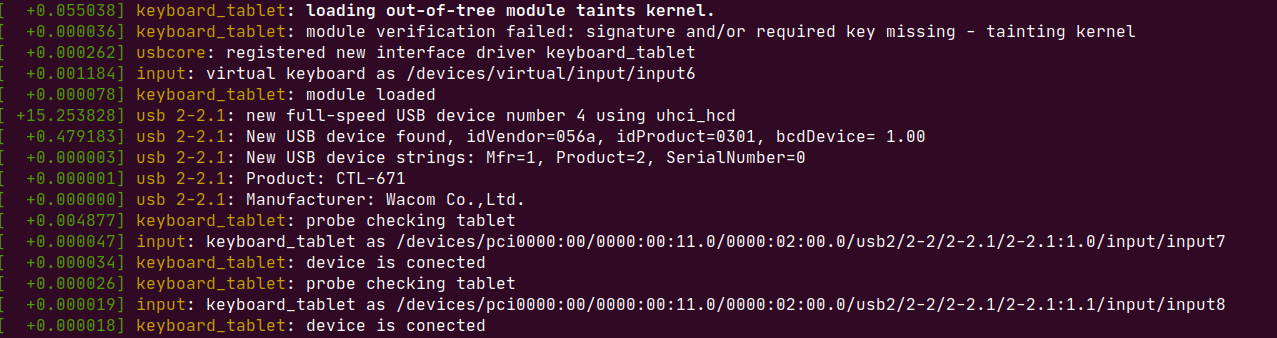
\includegraphics[width=0.8\textwidth]{img/connect.png}
    \caption{Подключение планшета к операционной системе}
    \label{fig:connect}
\end{figure}

На рисунке \ref{fig:work} изображены логи нажатий на планшет в разных областях.

\begin{figure}[H]
    \centering
    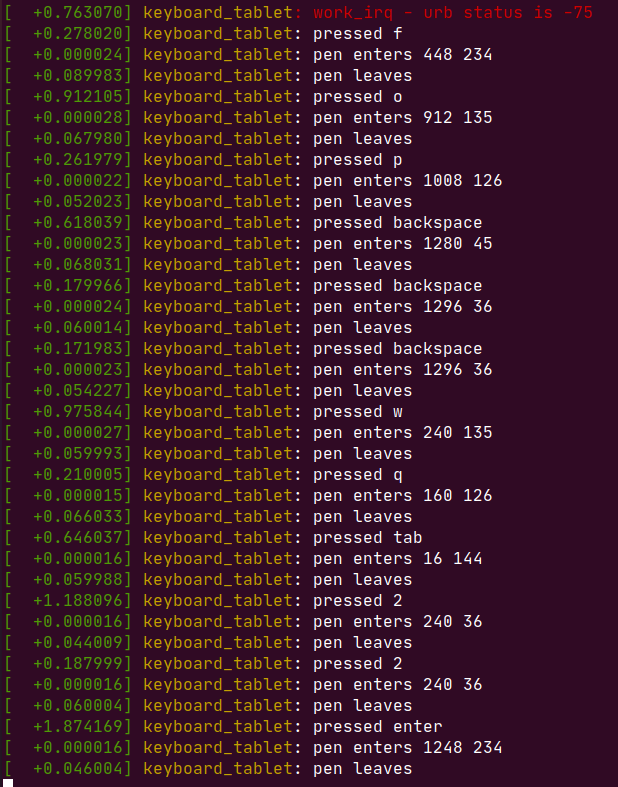
\includegraphics[width=0.8\textwidth]{img/work.png}
    \caption{Логи нажатий на планшет}
    \label{fig:work}
\end{figure}

На рисунке \ref{fig:work_wletters} изображены логи нажатий на планшет, когда открыта консоль с выводом логов. Здесь можно заметить перед сообщением о печати буквы сами эти буквы, которые были напечатаны с помощью планшета.

\begin{figure}[H]
    \centering
    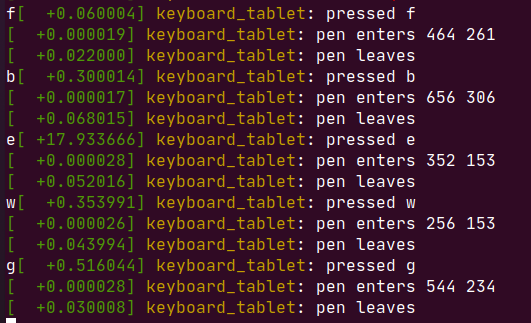
\includegraphics[width=0.8\textwidth]{img/work_wletters.png}
    \caption{Логи нажатий на планшет в консоли с логами}
    \label{fig:work_wletters}
\end{figure}

На рисунке \ref{fig:disconnect} изображены логи отключения планшета.

\begin{figure}[H]
    \centering
    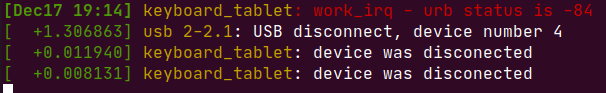
\includegraphics[width=0.8\textwidth]{img/disconnect.png}
    \caption{Отключение планшета от оперционной системы}
    \label{fig:disconnect}
\end{figure}

\section{Вывод}

В данном разделе был выбран язык программирования C, а также рассмотрена реализация программного обеспечения.
